\documentclass{article}

% Enumerator setting
\usepackage{enumerate}
\usepackage{enumitem}

% Language setting
% Replace `english' with e.g. `spanish' to change the document language
\usepackage[english]{babel}

% Set page size and margins
% Replace `letterpaper' with`a4paper' for UK/EU standard size
\usepackage[letterpaper,top=2cm,bottom=2cm,left=3cm,right=3cm,marginparwidth=1.75cm]{geometry}

% Useful packages
\usepackage{amssymb} % for \mathbb{R}
\usepackage{amsthm} % for proof
\usepackage{amsmath}
\usepackage{graphicx}
\usepackage[colorlinks=true, allcolors=blue]{hyperref}
\bibliographystyle{ieeetr}

% no indent for the whole document
\setlength\parindent{10pt}

\begin{document}
% \maketitle
\thispagestyle{plain}
\begin{center}
    \Large
    \textbf{Efficiency comparison of DDP and SQP on trajectory optimization}
        
    \vspace{0.4cm}
    \large
    ISEN 623 Final Report
        
    \vspace{0.4cm}
    \textbf{Ta-Wei Yeh (twy359)}
\end{center}

% ======= Abstract =======
\section{Abstract}
Trajectory optimization is an optimal control problem that outputs an optimal control trajectory considering a dynamical system over a period of time.  It is usually a nonlinear optimization problem, since the dynamical system and physical constraints are generally nonlinear in the real world. We select two optimal control solvers for comparison. The first solver is Sequential Quadratic Programming (SQP), and the second solver is Differential Dynamic Programming (DDP). When applying SQP to the control problem, the system dynamic model needs to be discretized over the whole trajectory which makes the problem dimension larger. In the conclusion, we showed that DDP is more efficient than SQP in terms of computation time. 

% ======= Introduction ========
\section{Introduction}
Trajectory optimization is an optimal control problem that optimizes the control input over the entire trajectory. A sequence of system states composed a trajectory. Each state is the consequent result from the control input and the system dynamics at each time step. In an optimal control problem, the decision variables need to consider the sysetm dynamics constraint which could easily be nonlinear in the real world. There are many methods to solve an optimal control problem. In general, we can divide the methods into two categories, classical and alternative. There are direct, indirect, and dynamic programming methods in the classical methods. Whereas alternative methods included learning-based and geometric methods to name a few. 
\begin{figure}[h]
    \centering
    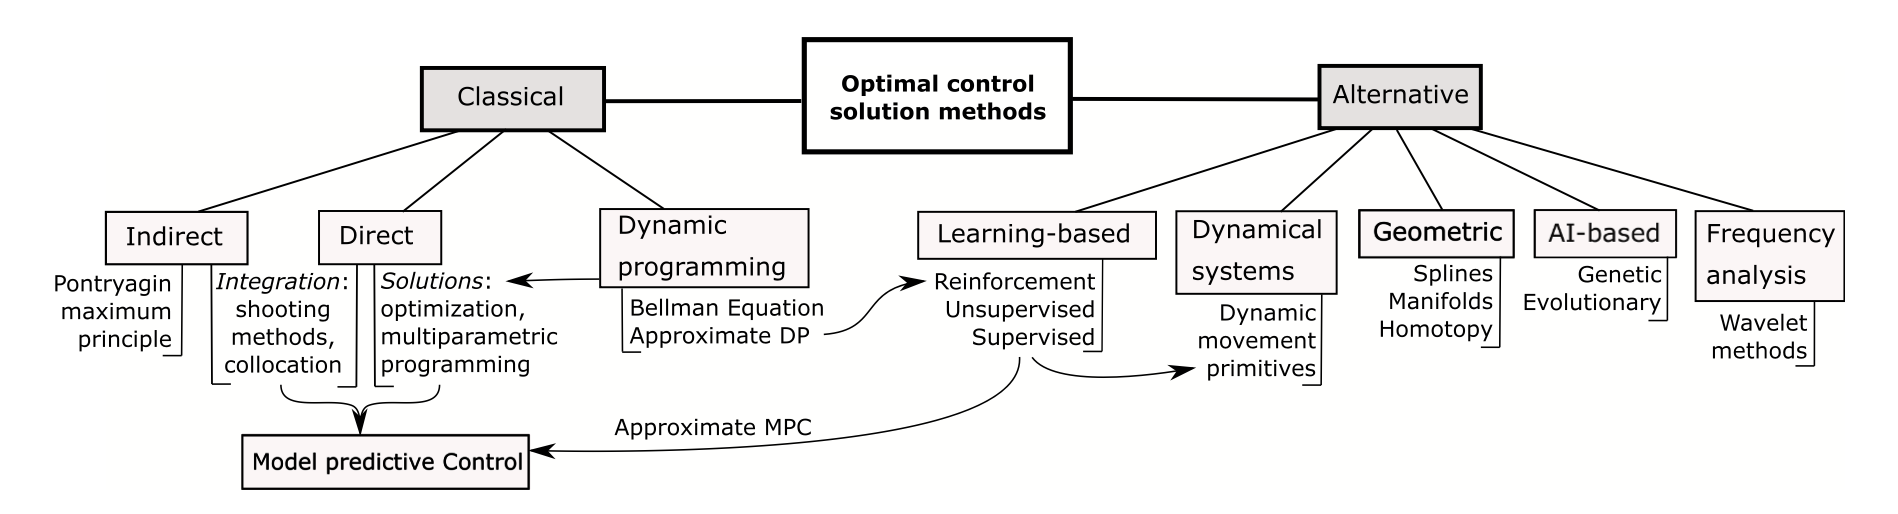
\includegraphics[width=\textwidth]{images/Approximate-taxonomy-of-optimal-control-solution-methods.png}
    \caption{Approximate taxonomy of optimal control solution methods \cite{optimal-control-taxonomy}}
    \label{fig:optimal-control-taxonomy}
\end{figure}

Now, we only focus on the classical methods that utilized well studied quadratic optimization solvers. In the direct method, Sequential Quadratic Programming (SQP) is widely adopted to the optimal control problem. In dynamic programming, Differential Dynamic Programming is considered because it reduces the problem dimension. Xie's Constraint Differential Dynamic Programming paper solves the control problem considering nonlinear constraints \cite{CDDP} which is included in the result for comparison. Both SQP and CDDP are nonlinear optimization solvers which could optimize not only nonlinear objective function but also nonlinear constraints. 

In the following sections, we will introduce the trajectory optimization problem and the two solvers, SQP and DDP. Finally, we will compare the efficiency of these two solvers in terms of computation time. 

% ======= Problem ========

\section{Problem}
\subsection{What is a trajectory optimization problem?}

A trajectory optimization problem is an optimal control problem that aims to find the optimal control inputs over a given time horizon to minimize a cost function while satisfying system dynamics and constraints. It involves finding the control inputs that result in the desired trajectory of a system while considering various constraints such as state bounds, control bounds, and path constraints. The goal is to find the control inputs that optimize a certain performance criterion, such as minimizing energy consumption or maximizing system stability.

Here is a figure \ref{fig:trajectory-optimization-with-obstacles} that simulates a car trajectory optimization problem. The car needs to reach the goal position while avoiding obstacles and minimizing the control effort. The trajectory optimization problem involves finding the optimal control inputs (steering angle, forward velocity) that guarantee the car to reach the final destination while satisfying the system dynamics and constraints.

\begin{figure}[h!]
    \centering
    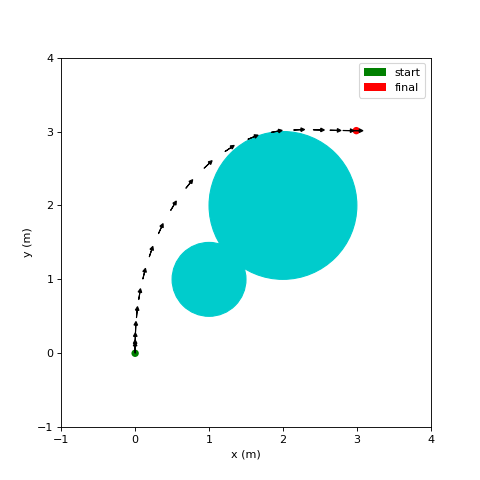
\includegraphics[width=0.5\textwidth]{images/with_obstacles.png}
    \caption{Trajectory optimization problem with obstacles}
    \label{fig:trajectory-optimization-with-obstacles}
\end{figure}

\subsection{Problem Formulation}
The trajectory optimization problem in continuous time can be formulated as follows:
\begin{align}
    \min_{\textbf{u}} \quad & \int^{T}_{t=0} l(\textbf{x}_t, \textbf{u}_t) + l^f(\textbf{x}_{T}) \\
    s.t. \quad & \Dot{\textbf{x}_t} = f(\textbf{x}_t, \textbf{u}_t) \\
    & \textbf{x}_{t=0} = \textbf{x}_0 \\
    & g(\textbf{x}_t, \textbf{u}_t) \leq 0
\end{align}

where $l$ is the cost-to-go function, 
$l^f$ is the final cost function which considers the final state, 
$\textbf{x}_t$ is the state variables (e.g. positions and orientation) at time t, 
$\textbf{u}_t$ is the control input (e.g. forward speed and angular speed) at time t, 
$T$ is the total control time horizon, 
$f$ is the differential equation of the system dynamic model, 
$\textbf{x}_0$ is the initial state, and 
$g$ is the inequality constraint which could include trajectory obstacles. 

The goal is to minimize the trajectory cost function $l(x, u)$ within time horizon $T$ while satisfying the system dynamics $f(x, u)$ and constraints $g(x, u)$. The final cost function guarantee the final state reach the final position. The decision variables are the control inputs $\textbf{u}$. 

% ======= Methods ========
\section{Methods}
\subsection{Sequential Quadratic Programming (SQP)}

Sequential Quadratic Programming is an iterative method for solving nonlinear optimization problems. It is a direct method that requires the system dynamics to be discretized over the entire trajectory. The optimization problem is solved by iteratively solving a sequence of quadratic subproblems that approximate the original nonlinear problem. At each iteration, the objective function and constraints are approximated by a quadratic model, and the solution of the quadratic subproblem is used to update the current solution. The process is repeated until convergence is achieved.

In trajectory optimization problem, each system state is the output from the system dynamics given the control input at each time step. To integrate SQP with trajectory optimization, we need to discretize the dynamic function which is usually described by a differential equation. The trajectory is composed by a sequence of the system states and control inputs over the time horizon. There are three ways to discretize the system dynamics, single shooting, multiple shooting, and collocation. In the single shooting method, the control inputs are the decision variables. In the multiple shooting method (figure \ref{fig:multiple-shooting-system-dynamics}), the state variables and control inputs at each time step are the decision variables. In the collocation method \cite{collocation}, additional state variables are introduced to approximate the system dynamics. 

\begin{figure}[h!]
    \begin{minipage}{0.4\textwidth}
        \centering
        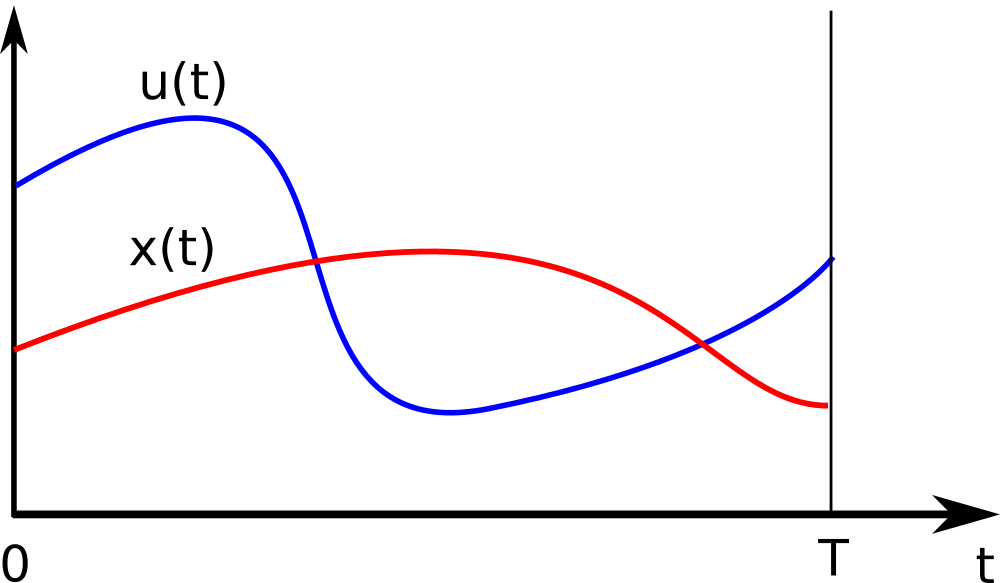
\includegraphics[width=\textwidth]{images/xu_cont.png}
        \caption{Continuous system dynamics}
        \label{fig:continuous-system-dynamics}
    \end{minipage}
    \hfill
    \begin{minipage}{0.4\textwidth}
        \centering
        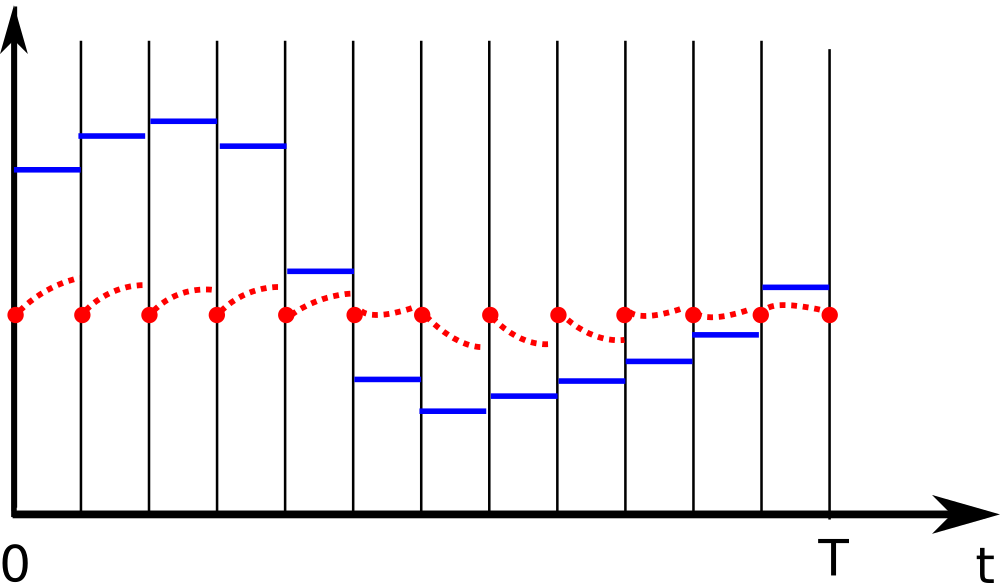
\includegraphics[width=\textwidth]{images/xu_gap.png}
        \caption{Multiple shooting discretized system dynamics}
        \label{fig:multiple-shooting-system-dynamics}
    \end{minipage}
    \label{fig:compare-system-dynamics}
\end{figure}

We decided to discretize the dynamic function with multiple shooting method since it is more accurate than single shooting method and easier to implement than collocation method. The optimization problem after discretization can be formulated as follows:
\begin{align}
    \min_{\textbf{x}, \textbf{u}} \quad & \sum^{N-1}_{k=0} l(\textbf{x}_k, \textbf{u}_k) + l^f(\textbf{x}_N) \\
    s.t. \quad & \textbf{x}_{k+1} = \textbf{x}_k + h \cdot f(\textbf{x}_{k}, \textbf{u}_{k}), \quad k = [0, N-1] \\
    & \textbf{x}_{k=0} = \textbf{x}_0 \\
    & g(\textbf{x}_k, \textbf{u}_k) \leq 0, \quad\quad k=[0, N]
\end{align}
where  $h$ is the time step, and $N$ is the time horizon given by $T/h$.

After discretization, the continuous system dynamics function (2) becomes (6) and the optimization problem becomes (5). The objective function discretizes the entire trajectory using multiple shooting methods. Optimizing over the entire trajectory rapidly increase the computational complexity \cite{lantoine2012hybrid} and causes problem dimension to be large making the optimization slower. Therefore, we are introducing the Differential Dynamic Programming (DDP) method to compare the efficiency. 

\subsection{Differential Dynamic Programming (DDP)}

Differential Dynamic Programming is a dynamic programming method that solves optimal control problems by iteratively approximating the value function and the optimal control policy. It is an indirect method that does not require the system dynamics to be discretized over the entire trajectory (9). Instead, it uses a local linearization of the system dynamics to compute the optimal control inputs at each time step. This is possible thanks to the Bellman's Optimal Principle which states that the optimal control policy only depends on the resulting states from the initial states. As a result, the value function over time horizon could be broken down into a sub-problem (10) at each time step. The sub-problem solves the optimal control input at each time step given the value function from the previous time step. 

\begin{align}
    V_k(\textbf{x}) & = \min_{\textbf{u}} \sum^{N-1}_{j=k} l(\textbf{x}_j, \textbf{u}_j) + l^f(\textbf{x}_N) \\
    & = \min_{\textbf{u}} l(\textbf{x}_k, \textbf{u}) + V_{k+1}(f(\textbf{x}, \textbf{u})) 
\end{align}
where the boundary condition is $V_N(x) = l^f(x)$. 

The optimization solves backward from time step $T$ to 0 which is called backward pass. The backward pass determined the step directions of a nominal trajectory. However, the trajectory might violate the constraints. Thus, in the forward pass, it ensures the trajectory feasibility is satisfied and decrease the trajectory cost using a trust region method. The forward optimizaiton starts from time 0 to $T$. The backward and forward optimization repeats until the nominal trajectory is converged. 

\begin{figure}[h!]
    \centering
    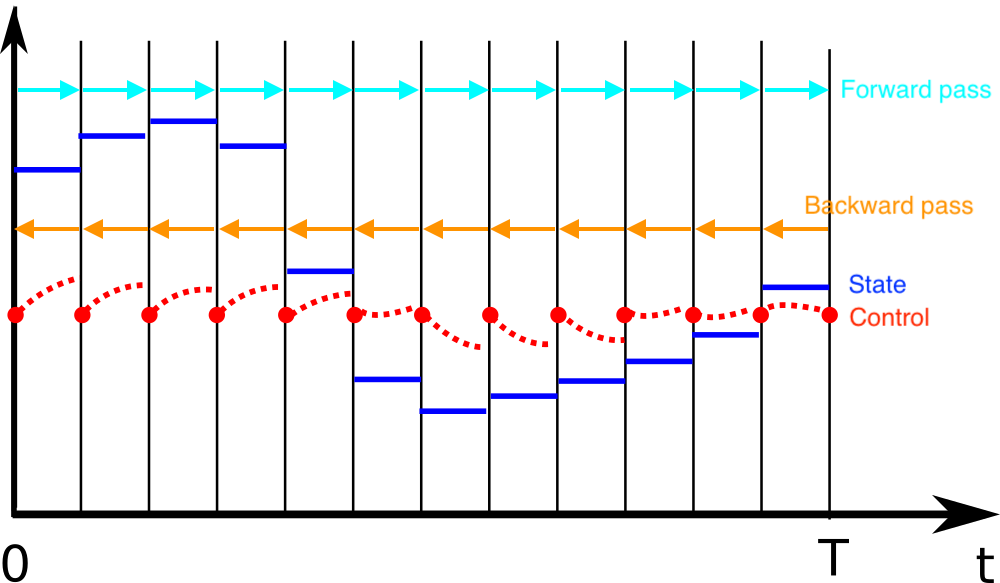
\includegraphics[width=0.4\textwidth]{images/xu_gap_ddp.png}
    \caption{Differential Dynamic Programming}
    \label{fig:ddp}
\end{figure}

% ======= Result ========
\section{Result}

The objective of the optimal control problem are the same for SQP and DDP which is driving a 2D car to reach the final destination while avoiding obstacles. To achieve this, the objective function is consisted of the trajectory cost function $l(x,u) = hu^TRu$ and the final cost function $l^f(x) = (x - x^{goal})^TQ^f(x-x_{goal})$, where $h$ is the time step, $R$ is a identity matrix, $Q^f$ is a diagonal matrix with larger diagonal values on car positions. The time horizon $T$ is 5 seconds and multiple shooting discretize the trajectory into 100 time steps. 

The 2D car follows the simplified vehicle dynamic in the CDDP paper \cite{CDDP}:

\begin{align*}
    x_{k+1} &= x_k + h v_k sin(\theta_k) \\
    y_{k+1} &= y_k + h v_k cos(\theta_k) \\
    \theta_{k+1} &= \theta_k + h u^{\theta} v_k \\
    v_{k+1} &= v_k + h u^{v} 
\end{align*}
where the state x = \{$x, y, \theta, v$\}, includes car position ($x, y$), car heading angle $\theta$, and forward velocity $v$. There are two control inputs which are angular velocity $u^{\theta}$, and forward velocity $u^k$. 

The implementation of Differential Dynamic Programming is pulled from Xie's CDDP GitHub repository \footnote{CDDP GitHub \url{https://github.com/ZhaomingXie/CDDP}.}. I implemented the trajectory optimization on SQP with multiple shooting method. To have a fare comparison, both programming languages are Python and execute under Apple M2 Silicon. The SQP solver is provided by SciPy, a free optimizer. I was trying to integrate SNOPT \cite{gill2005snopt}, a professional SQP solver, with Casadi \cite{andersson2019casadi}, a popular and free optimal control solver. However, it was not straightforward. If the integration was successful, the SQP computation result could have been faster since SNOPT considers objective function sparsity, Hessian, and Jacobian matrix. My code and instructions could be found in my course GitHub repository \footnote{ISEN623 Course Project \url{https://github.com/TaWeiYeh/ISEN-623-Project}}. 

The result figures \ref{fig:ddp-with-obstacles} and \ref{fig:sqp-with-obstacles} show the comparison between DDP and SQP on the trajectory optimization problem with obstacles. The computation time of DDP, 1.27 seconds, is significantly shorter than SQP, 71.97 seconds, thus the computation time of DDP is faster than SQP. 

\begin{figure}[h!]
    \begin{minipage}{0.4\textwidth}
        \centering
        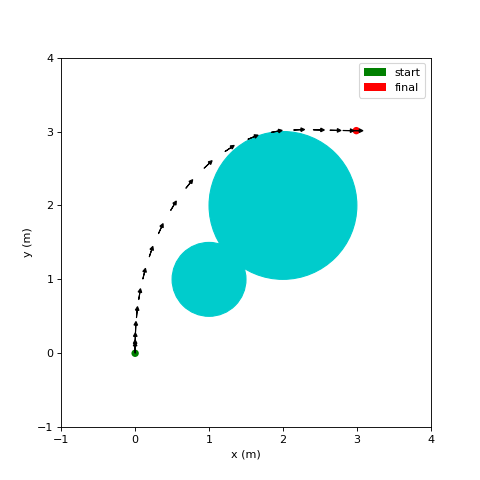
\includegraphics[width=\textwidth]{images/with_obstacles.png}
        \caption{DDP trajectory optimization with obstacles}
        \label{fig:ddp-with-obstacles}
    \end{minipage}
    \hfill
    \begin{minipage}{0.4\textwidth}
        \centering
        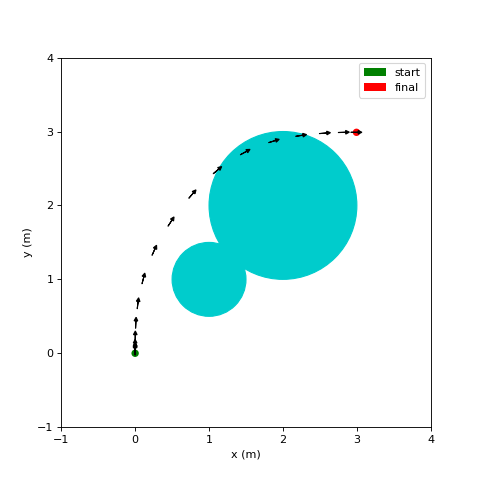
\includegraphics[width=\textwidth]{images/sqp_T5_constrained.png}
        \caption{SQP trajectory optimization with obstacles}
        \label{fig:sqp-with-obstacles}
    \end{minipage}
    \label{fig:two-figures}
\end{figure}


% ======= Conclusion ========
\section{Conclusion}

In conclusion, we compared the efficiency of two optimal control solvers, SQP and DDP, on the trajectory optimization problem. We found that DDP is more efficient than SQP in terms of computation time. The result shows that DDP solves faster than SQP and requires less computation time to solve the trajectory optimization problem. Therefore, DDP is a more efficient solver for trajectory optimization problems with nonlinear dynamics and constraints.

The conclusion could be exaggerated since the SQP solver could be optimized based on the objective function Hessian and Jacobian matrix. Also, the matrix sparsity could be utilized by the professional SQP optimizer, SNOPT \cite{gill2005snopt}. The comparison could be more accurate if the professional optimizer is used for the SQP solver.

Nonetheless, the optimization dimension problem is discussed by Xie \cite{CDDP} and Lantoine \cite{lantoine2012hybrid}. SQP suffers from the problem dimension whereas Dynamic Programming overcomes the "curse of dimensionality" of pure dynamic programming. Thus, I believe DDP would be an efficient solver when it comes to a trajectory optimization problem. 

% ======= References ========

\nocite{*} 
\bibliography{refs} % Entries are in the refs.bib file

\end{document}
